\documentclass[12pt]{article}

\usepackage{amsmath,amsthm}
\usepackage{amsfonts}
\usepackage[psamsfonts]{amssymb}
\usepackage{palatino,euler}
\usepackage{graphicx}
\usepackage{hyperref}
\usepackage[french]{babel}
\usepackage{gensymb}
\usepackage{siunitx}
\usepackage[margin=1.25in]{geometry}
\usepackage{tikz}

\newcommand\critical{\SI{3.98}\celsius}
\numberwithin{figure}{section}

\title{MAT1460\\[3ex]Fermeture de la patinoire naturelle du Lac aux Castors}
\author{Chen, Siying\\[1ex] Labont\'e, Pierre-Luc\\[1ex]Higgins, Philip\\[1ex] Grenier, David}
\date{}
\begin{document}

\maketitle
\thispagestyle{empty}
\vfill
\begin{center}
Universit\'e de Montr\'eal

\today
\end{center}
\clearpage

\tableofcontents
\newpage
\section{Introduction}

Dans le cadre de travaux effectu\'es par la Ville de Montr\'eal au Lac aux Castors le probl\`eme de
polif\'eration d'algues a \'et\'e r\'egl\'e. Toutefois, la patinoire hivernale naturelle est
d\'esormais ferm\'ee en vertu d'un accident hivernale reli\'e \`a la qualit\'e de la glace. Les
citoyens ne pourront d\'esormais plus jouir de cette activit\'e au Lac aux Castors.

Le r\'echauffement plan\'etaire \'etant d\'esormais une r\'ealit\'e scientifiquement accept\'ee les
gestionnaires ont bl\^am\'e la situation sur des temp\'eratures plus \'elev\'ees qu'autrefois.
Toutefois, une cons\'equence directe des travaux est que la profondeur du lac a augment\'e de fa\c
con significative. Il est donc possible qu'il soit tout simplement plus difficile d'obtenir une
\'epaisseur de glace suffisante en raison du volume d'eau plus important \`a refroidir.

Nous avons donc construit certains mod\`eles permetant de v\'erifier l'impact des raisons
ci-haut mentionn\'es sur la qualit\'e de la glace.

\section{Impact de la temp\'erature}

Nous ne crayons pas \^etre en mesure de r\'epondre de fa\c con satisfaisante \`a la r\'ealit\'e du
r\'echauffement plan\'etaire. Nous pensons toutefois v\'erifier le bienfond\'e de l'argument de la
Ville de Montr\'eal sur la cause ultime de l'accident de l'hiver 2016-2017 qui est survenu apr\`es
les travaux de r\'efections.

Nous allons d'abord d\'eterminer si il y a une diff\'erence statistiquement significative dans les
temp\'eratures enregistr\'ees aux cours des ann\'ees r\'ecentes \`a celles historiques. Il est
entendu que la condition de la glace d\'epend des temp\'eratures ext\'erieures et nous allons donc
aussi tenter de mesurer le niveau de corr\'elation entre les temp\'eratures observ\'ees et les
donn\'es d'ouverture des patinoires de l'\^Ile de Montr\'eal~\cite{PatHist}.

\subsection{Hypoth\`eses}

Nos hypoth\`eses sont principalement ax\'ees sur la nature des donn\'ees que nous avons recueillies:

\begin{enumerate}
    \item On suppose que nos donn\'ees sur les temp\'eratures recueillies sont uniform\'ement
        distribu\'ees \`a Montr\'eal;
    \item Lorsque les donn\'ees sont absentes en d\'ebut d\'ecembre et fin mars, nous supponsons que
        les patinoires sont ferm\'ees et que nous sommes hors-saison;
    \item Nous consid\'erons que les donn\'es accumul\'ees sur les conditions des patinoires sont
        fiables;
    \item Nous assumons que l'\'ecart-type de temp\'erature donn\'ee par le minist\`ere est
        l'\'ecart-type r\'eel des temp\'eratures d'hivers avec lesquels nous comparons~\cite{AvgTemp};
    \item On suppose que s'il y a effectivement r\'echauffement plan\'etaire que ce dernier
        n'affecte pas significativement l'\'ecart-type.
\end{enumerate}

\subsection{Augmentation de la temp\'erature}

En utilisant les donn\'es de temp\'eratures disponible~\cite{TempHist} nous avons effectu\'e un test
d'hypoth\`ese pour d\'eterminer si les temp\'eratures moyennes des 10 derni\`eres ann\'ees \`a
celles des 30 derni\`eres ann\'ees compil\'ees par M\'et\'eoM\'edia~\cite{MeteoTemp}.

Notre test d'hypoth\`ese repose sur les variables suivantes:

\begin{table}[h]
    \centering
    \begin{tabular}{|l|l|r|}\hline
        Variable &Description &Valeur\\\hline
        $\mu_T$ &Moyenne de temp\'erature d\'ecembre-mars, 1981-2010 &-\SI{6.800}\celsius\\\hline
        $\sigma_T^2$, $\sigma_t^2$ &\'Ecart-type donn\'e par le minist\`ere &\SI{2.25}\celsius\\\hline
        $\mu_t$ &Moyenne \'echantillonnale d\'ecembre-mars, 2008-2017 &-\SI{5.062}\celsius\\\hline
        $n_T$ &Ann\'ees de temp\'eratures historique enregistr\'ees &30\\\hline
        $n_t$ &Ann\'ees de temp\'eratures r\'ecentes &10\\\hline
    \end{tabular}
\end{table}
\begin{align*}
    H_0&: \mu_T - \mu_t = 0\\
    H_A&: \mu_T - \mu_t < 0\\
    p_\text{valeur} &= \frac{\mu_T - \mu_t}{\sqrt{\frac{\sigma_T^2}{n_T} + \frac{\sigma_t^2}{n_t}}} = \frac{\mu_T - \mu_t}{\sigma_T\sqrt{\frac1{n_T}+\frac1{n_t}}}\\
                    &= \frac{-6.8 + 5.062}{\sqrt{2.25}\sqrt{\frac1{30}+\frac1{10}}} = -3.17
\end{align*}

Notre statistique de test \'etant tr\`es faible nous devons \'ecarter l'hypoth\`ese que les
temp\'eratures r\'ecentes ne sont pas sup\'erieures aux temp\'eratures historique.

Nous avons aussi extrait les donn\'ees d'ouverture des patinoires de l'\^Ile de Montr\'eal. Nous
avons concentr\'e nos efforts sur les donn\'ees des saisons 2008 \`a 2013, ann\'ees pour lesquels
nous avions les donn\'ees les plus robustes et ce pour les mois de D\'ecembre \`a Mars.

Nous avons \'etablis deux mesures pour v\'erifier la corr\'elation entre les temp\'eratures
observ\'ees et l'ouverture des patinoire. Notre premi\`ere pr\'ediction est le nombre de jours o\`u
la temp\'erature maximale est au plus \SI0\celsius. La seconde est plus complexe, on
ne comptabilisera une journ\'ee que si les crit\`eres suivants sont satisfaits:

\begin{enumerate}
    \item La temp\'erature moyenne de la journ\'ee est au plus \SI0\celsius;
    \item Une surface n'est patinable que si la journ\'ee est indirectement pr\'ec\'ed\'ee de deux
        nuits cons\'ecutives de temp\'eratures minimales d'au plus -\SI{10}\celsius;
    \item Indirectement signifie que la journ\'ee n'est pas s\'epar\'ee des nuits froides par
        trois jours cons\'ecutifs de temp\'erature moyenne sup\'erieure \`a \SI0\celsius.
\end{enumerate}

\begin{table}[h]
    \centering
    \begin{tabular}{|l|r|r|r|r|}\hline
        Ann\'ee &Temp moyenne &Pr\'ediction 1 &Pr\'ediction 2 &Ouvertures\\
                &(\si\celsius) & & &(nombre)\\\hline
        2017 &-4.92 &59 &82 &\\\hline
        2016 &-3.96 &52 &70 &\\\hline
        2015 &-6.69 &74 &89 &\\\hline
        2014 &-6.59 &72 &90 &\\\hline
        2013 &-5.05 &58 &61 &\\\hline
        2012 &-2.57 &50 &65 &57\\\hline
        2011 &-4.78 &66 &69 &56\\\hline
        2010 &-5.26 &65 &69 &55\\\hline
        2009 &-5.53 &72 &77 &62\\\hline
        2008 &-5.26 &61 &91 &62\\\hline
        Moyenne &-5.06 &62.0 &76.3 &58.4\\\hline
    \end{tabular}
\end{table}

On a trouv\'e une droite des moindres des moindres carr\'es entre nos deux pr\'edictions et les
temp\'eratures moyennes saisonni\`eres pour trouver leur corr\'elations. En particulier, la pr\'ediction
1 \`a une corr\'elation forte n\'egative $R = -0.892$.

\begin{figure}[h]
    \centering
    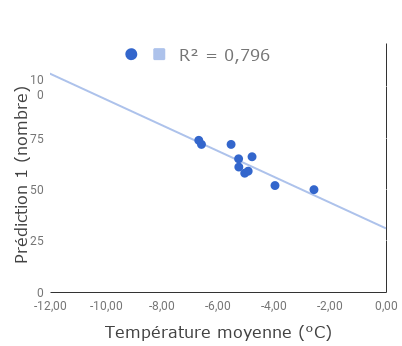
\includegraphics[scale=0.5]{Prediction1.png}
    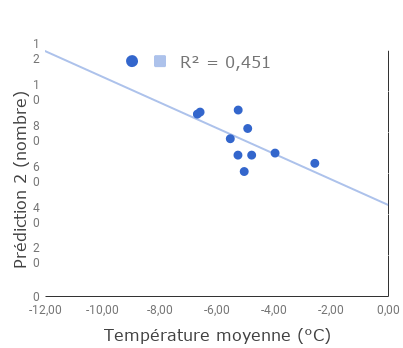
\includegraphics[scale=0.5]{Prediction2.png}
    \caption{Pr\'edictions 1 \& 2 contre les temp\'eratures moyennes saisonni\`eres}
\end{figure}

Nos pr\'edicteurs sont donc fortement reli\'es aux temp\'eratures moyennes saisonni\`eres, s'ils sont
efficaces pour pr\'edire les jours d'ouverture r\'eels on aura une bonne mesure de l'impact des
augmentations de temp\'eratures. On va v\'erifier si on doit rejeter la pr\'ediction 1 comme \'etant
une bonne repr\'esentation du nombre de jours d'ouvertures r\'eel en effectuant un test
d'hypoth\`ese d'une diff\'erence de moyenne. Puisque notre \'echantillon est petit nous allons
effectuer un test de Student soumises aux variables suivantes:

\begin{table}[h]
    \centering
    \begin{tabular}{|l|l|r|}\hline
        Variable &Description &Valeur\\\hline
        $n_1$, $n_2$ &Ann\'ees de donn\'es de patinoires ouvertes &5\\\hline
        $s$ &Estimateur de la diff\'erence de moyenne &\\\hline
        $s_1$, $s_2$ &\'Ecart-type \'echantillonnal &\\\hline
        $\overline{P_1}$ &Moyenne du pr\'edicteur 1 &\\\hline
        $\overline O$ &Moyenne des jours d'ouvertures &\\\hline
    \end{tabular}
    \caption{Variables pour les ann\'ees de donn\'ees pertinentes 2008-2012}
\end{table}

\begin{align*}
    s &= \sqrt{\frac{(n_1-1)s_1^2 + (n_2-1)s_2^2}{n_1+n_2-2}}\\
      &= \sqrt{39}\\
    T_{\overline{P_1}-\overline O} &= \frac{\overline{P_1} - \overline O}{s\sqrt{\frac1{n_1}+\frac1{n_2}}}
                                   = \frac{62.8-58.4}{\sqrt{39}\sqrt{\frac25}}\\
                                   &= 1.114
\end{align*}

On ne peut donc pas \'ecarter la possibilit\'e que notre $1^\text{er}$ pr\'edicteur est
repr\'esentatif des jours d'ouvertures r\'eel. L'\'equation de la droite des moindres carr\'es de la
pr\'ediction 1 est la suivante:

\[ y = -6.72x + 31.2 \]

Nous donne l'impact q'une augmentation d'un \si\celsius~va diminuer le nombre de jours d'ouvertures
d'environ 6.72 jours par ann\'ee. Les mod\`eles actuels nous disent que la temp\'erature globale
devrait augmenter de \SI4\celsius~d'ici 2100~\cite{GlobalRaise} par rapport \`a la temp\'erature
pr\'e-industrielle. Toutefois l'impact Canadien d'une telle augmentation serait le double de
l'impact global~\cite{CanadaRaise}. Nous interpr\'etons cette derni\`ere comme repr\'esentant une
augmentation d'environ \SI6\celsius~au cours des prochains 80 ans et donc une augmentation
\si{0.75}\celsius~par d\'ec\'enie.

\subsection{Validit\'e des r\'esultats}

\section{Impact de la profondeur}

Nous discuterons ici de l'effet de la profondeur du plan d'eau sur les conditions de glace. En
particulier, nous cherchons \`a savoir s'il est possible que d'avoir creus\'e~\cite{Lac} le lac \`a
contribu\'e \`a la fermeture de la patinoire pour assurer la s\'ecurit\'e du personnel et des
citoyens.

\subsection{Hypoth\`eses}

Afin de d\'eterminer l'impact de la profondeur d'un plan sur la formation de la glace nous allons
encadrer la question des simplifications suivantes:

\begin{enumerate}
    \item Quoique la temp\'erature ext\'erieure va normalement varier suite \`a la contribution
        en chaleur du lac, nous allons consid\'erer que les variations locales vont se distribuer
        et traiter l'environnement ext\'erieur comme un puit de chaleur.
    \item Similairement pour l'apport du lac et de l'air \`a la temp\'erature du sol et allons
        donc traiter le sol comme une source de chaleur in\'epuisable;
    \item Nous n'allons \'evaluer que la perte d'\'energie du lac en terme de la conduction thermique
        et consid\'erer les contributions en radiation et \'evaporation~\cite{Evap} des deux lacs
        identique;
    \item Nous allons supposer la temp\'erature ext\'erieure constante. (voir \ref{TempExt})
    \item Nous allons supposer la temp\'erature du sol constante et uniform\'ement distribu\'ee;
        (voir \ref{Conduc})
    \item Nous ne connaissons pas les conductivit\'e thermiques en surface et au fond du lac, mais
        nous allons les consid\'erer respectivement identiques pour nos deux lacs;
    \item Nous ne connaissons pas la nature de l'interface en surface et au fond du lac pour le
        calcul de flux thermique et par cons\'equent nous en ignoront l'\'epaisseur. Nous allons
        toutefois les consid\'erer respectivement identiques pour nos deux lacs.
\end{enumerate}

Nous tenterons donc de d\'eterminer, pour un plan d'eau d'une surface de superficie fixe, de quelle fa\c
con une augmentation de la profondeur (et donc du volume d'eau) va prolonger la p\'eriode n\'ecessaire
pour refroidir le lac. On comparera donc deux corps d'eau id\'ealis\'es et d\'elimit\'es par la m\^eme
surface circulaire, l'un plus profond que l'autre.

\subsubsection{Temp\'erature ext\'erieure constante}\label{TempExt}

Pour obtenir une r\'eponse r\'ealiste une simulation ou une utilisation judicieuse de probabilit\'es
nous permettrait d'inclure une fluctuation de temp\'erature. En particulier, nous savons que la
chaleur transmise entre deux corps est proportionnelle \`a la diff\'erence de temp\'erature entre
ces derniers~\cite{Fourier} et il serait pr\'eferable de ne pas n\'egliger cette composante.

Notre intuition nous dit qu'un lac dont le volume d'eau est sup\'erieur verra sa temp\'erature
varier plus lentement et que la diff\'erence de temp\'erature sera plus grande lorsque la
temp\'erature ext\'erieure est basse. Toutefois, il est important d'appr\'ecier que si tel est le
cas, lorsque la temp\'erature ext\'erieure passe au dessus de celle de nos deux lacs, la situation
est renvers\'ee et le lac dont le volume est inf\'erieur verra sa temp\'erature remonter plus
rapidement aussi.

Nous jugeons donc qu'il est raisonnable de supposer la temp\'erature ext\'erieure constante. Les
composantes de gains et pertes en chaleur dues \`a la variation de temp\'erature vont possiblement
s'annuler. Si ce n'est pas le cas et que le lac plus profond a une diff\'erence de temp\'erature
avec l'ext\'erieure plus grande on aura tout de m\^eme une r\'eponse positive \`a la question (que
le lac plus profond prends plus de temps \`a geler) en ayant possiblement surestim\'e l'impact de
la profondeur.

\subsection{La convection thermique}\label{Convec}

Puisque nous \'evaluerons la diminution de la temp\'erature d'un lac par la chaleur d\'egag\'ee par
le plan d'eau \`a l'air environnant il s'ensuit que la temp\'erature chutera en surface. La
capacit\'e thermique~\cite{CapTherm} massique du sol est inf\'erieure a celle de l'eau, toutefois le
volume de la terre est de loin sup\'erieur \`a celle d'un lac. On pourra ainsi supposer que la
temp\'erature du sol va demeurer sup\'erieure \`a celle de l'eau par temps froid ce qui justifie de
traiter le sol comme une source de chaleur.

\begin{figure}[h]\label{water-density}
    \centering
    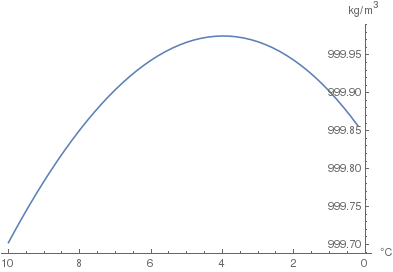
\includegraphics[scale=0.7]{WaterDensity.png}
    \caption{Densit\'e de l'eau}
\end{figure}

Une particularit\'e de l'eau est que sa densit\'e augmente avec une diminution de
temp\'erature~\cite{WaterDensity} et atteint son maximum \`a \critical~(voir figure
\ref{water-density}) ce qui introduit un processus de convection thermique~\cite{ConvNat}. Tant que
la temp\'erature du lac est sup\'erieure \`a \critical, l'eau qui refroidit \`a la surface va
sombrer et sera remplac\'ee par de l'eau plus chaude provenant pr\`es de la terre, l\`a o\`u la
temp\'erature est plus \'elev\'ee.

\begin{figure}[h]\label{water-convection}
    \centering
    \begin{tikzpicture}[scale=0.7]
        \shade[top color=blue!70,bottom color=brown] (0,5) -- (0,2) arc (180:360:3 and 0.5) -- (6,5)
        arc (0:180:3 and 0.5);
        \draw [<->] (3,5) -- (5.9,5) node [midway, above, scale=0.7] {$r$};
        \draw [<->] (6.3,5) -- (6.3,2) node [midway, right, scale=0.7] {$p_1$};
        \draw (3,5) ellipse (3 and 0.5);
        \draw (0,5) -- (0,2);
        \draw (6,5) -- (6,2);
        \draw [dashed] (0,2) arc (180:0:3 and 0.5);
        \draw (0,2) arc (180:360:3 and 0.5);
        \draw[line width=0.5mm, ->] (1.8,4.1) arc (95:445:1cm and 1cm);
        \draw[line width=0.5mm, ->] (4.2,4.1) arc (85:-260:1cm and 1cm);

        \shade[top color=blue!70,bottom color=brown] (7,5) -- (7,-4) arc (180:360:3 and 0.5) -- (13,5)
        arc (0:180:3 and 0.5);
        \draw [<->] (10,5) -- (12.9,5) node [midway, above, scale=0.7] {$r$};
        \draw [<->] (13.3,5) -- (13.3,-4) node [midway, right, scale=0.7] {$p_2$};
        \draw (10,5) ellipse (3 and 0.5);
        \draw (7,5) -- (7,-4);
        \draw (13,5) -- (13,-4);
        \draw [dashed] (7,2) arc (180:360:3 and 0.5);
        \draw [dashed] (7,-4) arc (180:0:3 and 0.5);
        \draw (7,-4) arc (180:360:3 and 0.5);
        \draw[line width=0.5mm, ->] (8.8,4.1) arc (95:445:1cm and 4cm);
        \draw[line width=0.5mm, ->] (11.2,4.1) arc (85:-260:1cm and 4cm);
    \end{tikzpicture}
    \caption{Convection \`a plus de \critical}
\end{figure}

Nous allons donc consid\'erer qu'un lac dont la temp\'erature est sup\'erieur \`a \critical, va voir
sa temp\'erature va diminuer de fa\c con \`a ce que l'eau demeure \`a temp\'erature uniforme.
D\'eterminer l'impact de la profondeur d'un lac pour diminuer sa temp\'erature \`a \critical~revient
donc \`a mesurer le temps n\'ecessaire pour obtenir les chaleurs respectives d\'egag\'ees.

\subsection{La conduction thermique (ou diffusion)}\label{Conduc}

Le sol \'etant un solide il n'est pas sujet \`a la convection tel l'eau du lac. Nous aurions une
meilleure approximation en consid\'erant le processus de diffusion qui, \`a un \'etat eventuel
stable, conduirait \`a une temp\'erature du sol lin\'eairement distribu\'ee~\cite{TempLinear}.
Toutefois, ces calculs seraient compliqu\'es et nous pensons pouvoir d\'eduire, par le th\'eor\`eme
de la moyenne~\cite{AvgValue}, qu'il existe une temp\'erature constante pour laquelle la
contribution en chaleur du sol sera la m\^eme que pour une temp\'erature distribu\'ee de fa\c con
plus r\'ealiste.

Remarquons aussi qu'en dessous de \critical, la densit\'e de l'eau se met \`a diminuer avec une
diminution de temp\'erature. Le processus de convection devient alors stable~\cite{HydroStab} et la
temp\'erature ne varie plus de fa\c con uniforme. On penses que la temp\'erature variera \`a
l'int\'erieur du corps tel la diffusion de la chaleur dans une tige, la profondeur aura donc quand
m\^eme un impact. Toutefois, il n'est plus n\'ecessaire \`a cette \'etape de refroidir le lac dans
son ensemble pour obtenir une formation de glace \`a la surface. Le refroidissement du lac doit donc
\^etre trait\'e diff\'eremment apr\`es l'atteinte de la temp\'erature uniforme de \critical.

\subsection{Mod\'elisation}

Nous introduisons les variables dont nous allons avoir besoin:

\begin{table}[h]
    \centering
    \begin{tabular}{|l|l|l|}\hline
        Variable &Description &Unit\'e\\\hline
        $Q$ &Chaleur &\si\joule\ (\si{\kilogram.\square\meter\per{\square\second}})\\\hline
        $T$ &Temp\'erature &\si{\kelvin}\\\hline
        $c_p$ &Capacit\'e thermique massique &\si{\joule\per{\kelvin\,\kilogram}}\\\hline
        $m$ &Masse &\si\kg\\\hline
        $C$ &Capacit\'e thermique &\si{\joule\per\kelvin}\\\hline
        $K$ &Conductivit\'e thermique &\si{\joule\per{\meter\,\second\,\kelvin}}\\\hline
        $\rho$ &Densit\'e de la substance &\si{\kilogram\per{\square\meter}}\\\hline
        $V$ &Volume &\si{\cubic\meter}\\\hline
        $r$ &Rayon d'un lac cylindrique &\si\meter\\\hline
        $A$ &Superficie &\si{\square\meter}\\\hline
        $p$ &Profondeur d'un lac cylindrique &\si\meter\\\hline
        $t$ &Temps &\si\second\\\hline
    \end{tabular}
    \caption{Variables}
\end{table}

Lorsqu'un corps subit une variation de temp\'erature $\Delta T$ l'energie transf\'er\'ee (chaleur)~\cite{Q-equation}
nous est donn\'e par:

\begin{align}
    Q &= C\Delta T\label{eq:heat}\\
    &= c_pm\Delta T\notag\\
    &= c_p\rho V\Delta T\notag\\
    &= c_p\rho (p\pi r^2p)\Delta T &&\text{(pour un lac cylindrique)}\notag
\end{align}

En particulier, la capacit\'e thermique d'un corps $(C)$ est une propri\'et\'e
extensive~\cite{Extensive} ce qui signifie que sa valeur est directement proportionnelle \`a la
taille du syst\`eme. On voit donc que si la masse du second lac est le triple du premier, il devra
perdre trois fois plus d'\'energie pour atteindre la m\^eme temp\'erature. Nous avons donc d\'ej\`a
une excellente raison de croire qu'une augmentation de la profondeur d'un lac sans augmentation de
sa surface aura un impact important sur le temps de refroidissement.

La figure \ref{water-convection} nous montre un second lac expos\'e \`a la m\^eme surface
ext\'erieure. Par contre, il est expos\'e \`a une plus grande superficie en contact avec le sol que
nous consid\'erons comme une source de chaleur. Nous allons donc \'evaluer d'un premier temps le
temps n\'ecessaire pour obtenir le d\'egagement de chaleur \`a l'atteinte de \critical.

Les donn\'ees officielles sur la superficie et la profondeur du Lac aux Castors semblent difficile
\`a obtenir. Nous avons toutefois r\'eussi \`a estimer la superficie du lac \`a environ
\SI{18500}{\square\meter} (voir figure \ref{google-castor}). On nous informe aussi qu'en vertu des travaux effectu\'es le lac est
pass\'e d'une profondeur d'environ 2 \`a 7 m\^etres~\cite{Lac-Castor}.

\begin{figure}\label{google-castor}
    \centering
    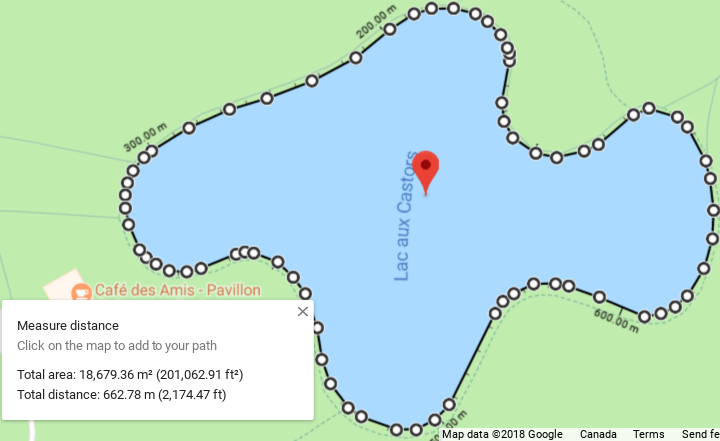
\includegraphics[scale=0.5]{Superficie.png}
    \caption{Superficie du Lac aux Castors}
\end{figure}

En ramenant ces donn\'ees \`a un lac cylindrique de superficie et volumes respectifs on obtient
les param\`etres ci-dessous pour effectuer nos calculs:

\begin{table}[h]
    \centering
    \begin{tabular}{|l|l|r|}\hline
        Param\`etre &Description &Valeur\\\hline
        $c_p$ &Capacit\'e thermique massique de l'eau &\SI{4185.5}{\joule\per{\kelvin\,\kilogram}}\\\hline
        $T_\text{sol}$ &Temp\'erature du sol &\SI{279.15}\kelvin\ (\SI8\celsius)\\\hline
        $T_\text{air}$ &Temp\'erature de l'air &\SI{261.15}\kelvin\ (\SI{-12}\celsius)\\\hline
        $T_\text{init}$ &Temp\'erature initiale de l'eau &\SI{285.15}\kelvin\ (\SI8\celsius)\\\hline
        $T_\text{cible}$ &Temp\'erature \`a hydrostabilit\'e &\SI{277.13}\kelvin\\\hline
        $A_{lac}$ &Superficie du lac &\SI{18500}{\square\meter}\\\hline
        $p_1,p_2$ &Profondeur du lac et lac excav\'e &\SI2\meter, \SI7\meter\\\hline
        $\rho$ &Densit\'e de l'eau &\SI1{\kilogram\per{\cubic\meter}}\\\hline
        $K$ &Conductivit\'e thermique de surface &inconnue\\\hline
        $x$ &\'Epaisseur de l'interface de surface &inconnue\\\hline
        $\alpha$ &Ratio des constantes du fond contre surface &param\`etre\\\hline
    \end{tabular}
    \caption{Param\`etres}
\end{table}
\clearpage

On trouves les pertes de chaleur n\'ecessaire de nos deux lacs:

\begin{align*}
    r &= \sqrt{\frac{18500}\pi} = \SI{76.738}\meter\\
    C_1 &= c_pm_1 = c_p\rho p_1\pi r^2 = \num{1.549e8}\si{\joule\per\kelvin}\\
    C_2 &= c_pm_2 = c_p\rho p_2\pi r^2 = \num{5.420e8}\si{\joule\per\kelvin}\\
    \Delta T &= T_\text{cible} - T_\text{init} = \SI{-4.02}\kelvin\\
    Q_1 &= C_1\Delta T = -\num{6.226e8}\si\joule\\
    Q_2 &= C_2\Delta T = -\num{2.179e9}\si\joule
\end{align*}

On doit maintenant \'evaluer la chaleur \'emise par la surface et re\c cue par le fond du lac.
L'\'equation du flux thermique \eqref{eq:flux} n'est normalement pas applicable
directement~\cite{HeatFlow} puisqu'elle est typiquement utilis\'ee entre deux syst\`emes de masse et
capacit\'e thermique massique identiques. Aussi, la structure des interfaces entre a surface de
l'eau et l'air ambiant ainsi que celle du fond du lac nous sont inconnues. Nous ne pensons pas
pouvoir trouver la conductivit\'e thermique appropri\'ee ainsi que le gradient de temp\'erature
r\'eel.

\begin{align}
    \frac{\Delta Q}{\Delta t} = -KA\frac{\Delta T}x \label{eq:flux}
\end{align}

Nous allons donc absorber ces constantes dans la variable d'int\'egration. Pour simplifier les
calculs nous allons aussi absorber l'aire de la surface et exprimer les constantes pour le fond du
lac comme le produit d'un nouveau param\`etre qu'on fera varier. Nous n'obtiendront donc pas une
unit\'e de temps r\'eelle mais nous allons toutefois \^etre en mesure d'\'evaluer la diff\'erence
relative entre nos deux syst\`emes.

\begin{align}
    A_1 &= 2\pi r p_1 + \pi r^2 = \num{1.946e4}\si{\square\meter}\notag\\
    \frac{dQ_1}{dt} &=
        -KA_\text{lac}\frac{T_1(t) - T_\text{air}}x -\alpha KA_1\frac{T_\text{fond}-T_1(t)}x\notag\\
    &= \underbrace{KA_\text{lac}\frac{T_\text{air}-T_1(t)}x\
        -\alpha KA_1\frac{T_\text{fond}-T_1(t)}x}_{\tau = A_\text{lac}\frac Kxt}\notag\\
    \frac{dQ_1}{d\tau} &= T_\text{air} - T_1(\tau) - \alpha (T_\text{fond} -
        T_1(\tau))\label{eq:diff}\\
    \text{o\`u } T_1(\tau) &= T_\text{cible} - \frac{Q_1(\tau)}{C_1} \label{eq:temp}&&\text{(par l'\'equation \ref{eq:heat})}
\end{align}

En substituant \eqref{eq:temp} dans l'\'equation \eqref{eq:diff} on obtient une \'equation
diff\'erentielle \`a variable s\'eparable qui n'est pas si difficile \`a r\'esoudre. En donnant les
conditions initiales ($Q(0) = 0$) on trouves $Q_1(\tau)$ et $Q_2(\tau)$. Apr\`es substitution dans
\eqref{eq:temp} on obtient les \'equations nous donnant l'\'evolution de la temp\'erature en fonction
de notre temps $\tau$.

\begin{align*}
    T_1(\tau) &=
        T_\text{init} +
            \left(1-e^{\textstyle -t\frac{\alpha A_1-A_\text{lac}}{C_1}}\right)
            \frac
                {A_\text{lac} T_\text{air} + (\alpha A_1-A_\text{lac})T_\text{cible} - \alpha A_1 T_\text{fond}}
                {\alpha A_1-A_\text{lac}}\\
    T_2(\tau) &=
        T_\text{init} +
            \left(1-e^{\textstyle -t\frac{\alpha A_2-A_\text{lac}}{C_2}}\right)
            \frac
                {A_\text{lac} T_\text{air} + (\alpha A_2-A_\text{lac})T_\text{cible} - \alpha A_2 T_\text{fond}}
                {\alpha A_2-A_\text{lac}}\\
\end{align*}

Ces derni\`eres \'etant inversibles, on a pu trouver le temps $\tau$ pour atteindre la perte de
chaleur recherch\'ee pour diverses valeurs de $\alpha$. On trace ainsi les courbes des chutes de
temp\'eratures pour les deux lacs.

\begin{figure}
    \centering
    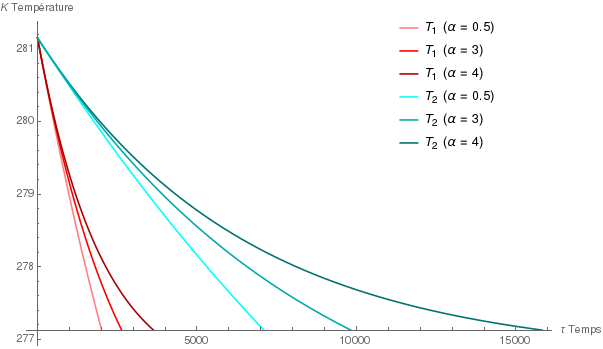
\includegraphics[scale=0.7]{Alpha.png}
    \caption{Chutes de temp\'eratures pour $\alpha \in \{0.5, 3, 4\}$.}
\end{figure}

\subsection{Validit\'e des r\'esultats}

\section{Analyse}
\subsection{Discussion des r\'esultats}
\subsection{Forces et faiblesses}

\section{Conclusion}

\clearpage
\section{Bibliographie}
\begin{thebibliography}{Xyz}
    \bibitem{TempHist} \href{https://www.meteomedia.com/ca/api/sitewrapper/index?b=%2Fstatistics%2F&p=%2Fprevisions%2Fstatistiques%2Findex&url=%2Fstatistics%2Fcaqc0363%2Fmontreal%2F%2F%2F%3F}
        {M\'et\'eoM\'edia - Montr\'eal}
    \bibitem{PatHist} \href{http://donnees.ville.montreal.qc.ca/dataset/patinoires-historique}
        {Patinoire - historique des conditions}
    \bibitem{AvgTemp} \href{http://www.mddelcc.gouv.qc.ca/climat/surveillance/classification.htm}
        {Classification climatologique des temp\'eratures}
    \bibitem{MeteoTemp} \href{https://www.meteomedia.com/ca/api/sitewrapper/index?b=%2Fstatistics%2F&p=%2Fprevisions%2Fstatistiques%2Findex&url=%2Fstatistics%2Fcaqc0363%2Fmontreal%2F%2F%2F%3F}
            {Statistiques: Montr\'eal, Que\'ebec - M\'et\'eoM\'edia}
    \bibitem{GlobalRaise} \href{https://www.independent.co.uk/environment/global-warming-temperature-rise-climate-change-end-century-science-a8095591.html}
        {Worst-case global warming predictions}
    \bibitem{CanadaRaise} \href{https://www.canada.ca/fr/environnement-changement-climatique/services/changements-climatiques/science.html}
        {Science des changements climatiques}
    \bibitem{Lac} \href{https://www.ledevoir.com/politique/montreal/517828/patinoire-du-lac-aux-castors}
        {Montr\'eal abandonne la patinoire naturelle du lac aux Castors}
    \bibitem{Evap} \href{https://www.quora.com/How-does-evaporation-take-place-at-all-temperatures-whereas-boiling-takes-place-at-a-fixed-temperature-under-a-given-pressure}
        {How does evaporation take place at all temperatures}
    \bibitem{Fourier} \href{https://fr.wikipedia.org/wiki/Conduction_thermique#Loi_de_Fourier}
        {Loi de Fourier}
    \bibitem{CapTherm} \href{https://fr.wikipedia.org/wiki/Capacit%C3%A9_thermique_massique}
        {Capacit\'e thermique massique}
    \bibitem{WaterDensity} \href{http://www.open.edu/openlearn/science-maths-technology/the-oceans/content-section-3.2}
        {The density of fresh water and seawater}
    \bibitem{ConvNat} \href{https://fr.wikipedia.org/wiki/Convection_thermique#Convection_naturelle}
        {Convection naturelle}
    \bibitem{TempLinear} \href{https://fr.wikipedia.org/wiki/Conduction_thermique#Surfaces_planes_en_série}
        {Conduction Thermique - Profil des temp\'eratures}
    \bibitem{AvgValue} \href{https://fr.wikipedia.org/wiki/Th%C3%A9or%C3%A8me_de_la_moyenne}
        {Th\'eor\`eme de la moyenne}
    \bibitem{HydroStab} \href{https://fr.wikipedia.org/wiki/Gradient_thermique_adiabatique#Atmosph.C3.A8re_stable}
        {Stabilit\'e hydrostatique}
    \bibitem{Q-equation} \href{https://simple.wikipedia.org/wiki/Specific_heat#Usage}
        {Calculating heat}
    \bibitem{Extensive} \href{https://fr.wikipedia.org/wiki/Extensivit%C3%A9_et_intensivit%C3%A9_(physique)}
        {Extensivit\'e}
    \bibitem{Lac-Castor} \href{https://fr.wikipedia.org/wiki/Lac_aux_Castors_(Montr%C3%A9al)}
        {Lac aux Castors}
    \bibitem{SpecHeat} \href{https://www.engineeringtoolbox.com/specific-heat-capacity-d_391.html}
        {Specific heat of common Substances}
    \bibitem{NewtonLaw} \href{https://en.wikipedia.org/wiki/Newton%27s_law_of_cooling}
        {Newton Law of cooling}
    \bibitem{HeatFlow} \href{https://en.wikipedia.org/wiki/Rate_of_heat_flow}
        {Rate of heat flow}
    \bibitem{Conductivity} \href{https://www.engineeringtoolbox.com/thermal-conductivity-d_429.html}
        {Thermal Conductivity of common Materials and Gases}
\end{thebibliography}

\end{document}
